\section{Component view}
\label{sec:component-view}

\begin{figure}
\centering
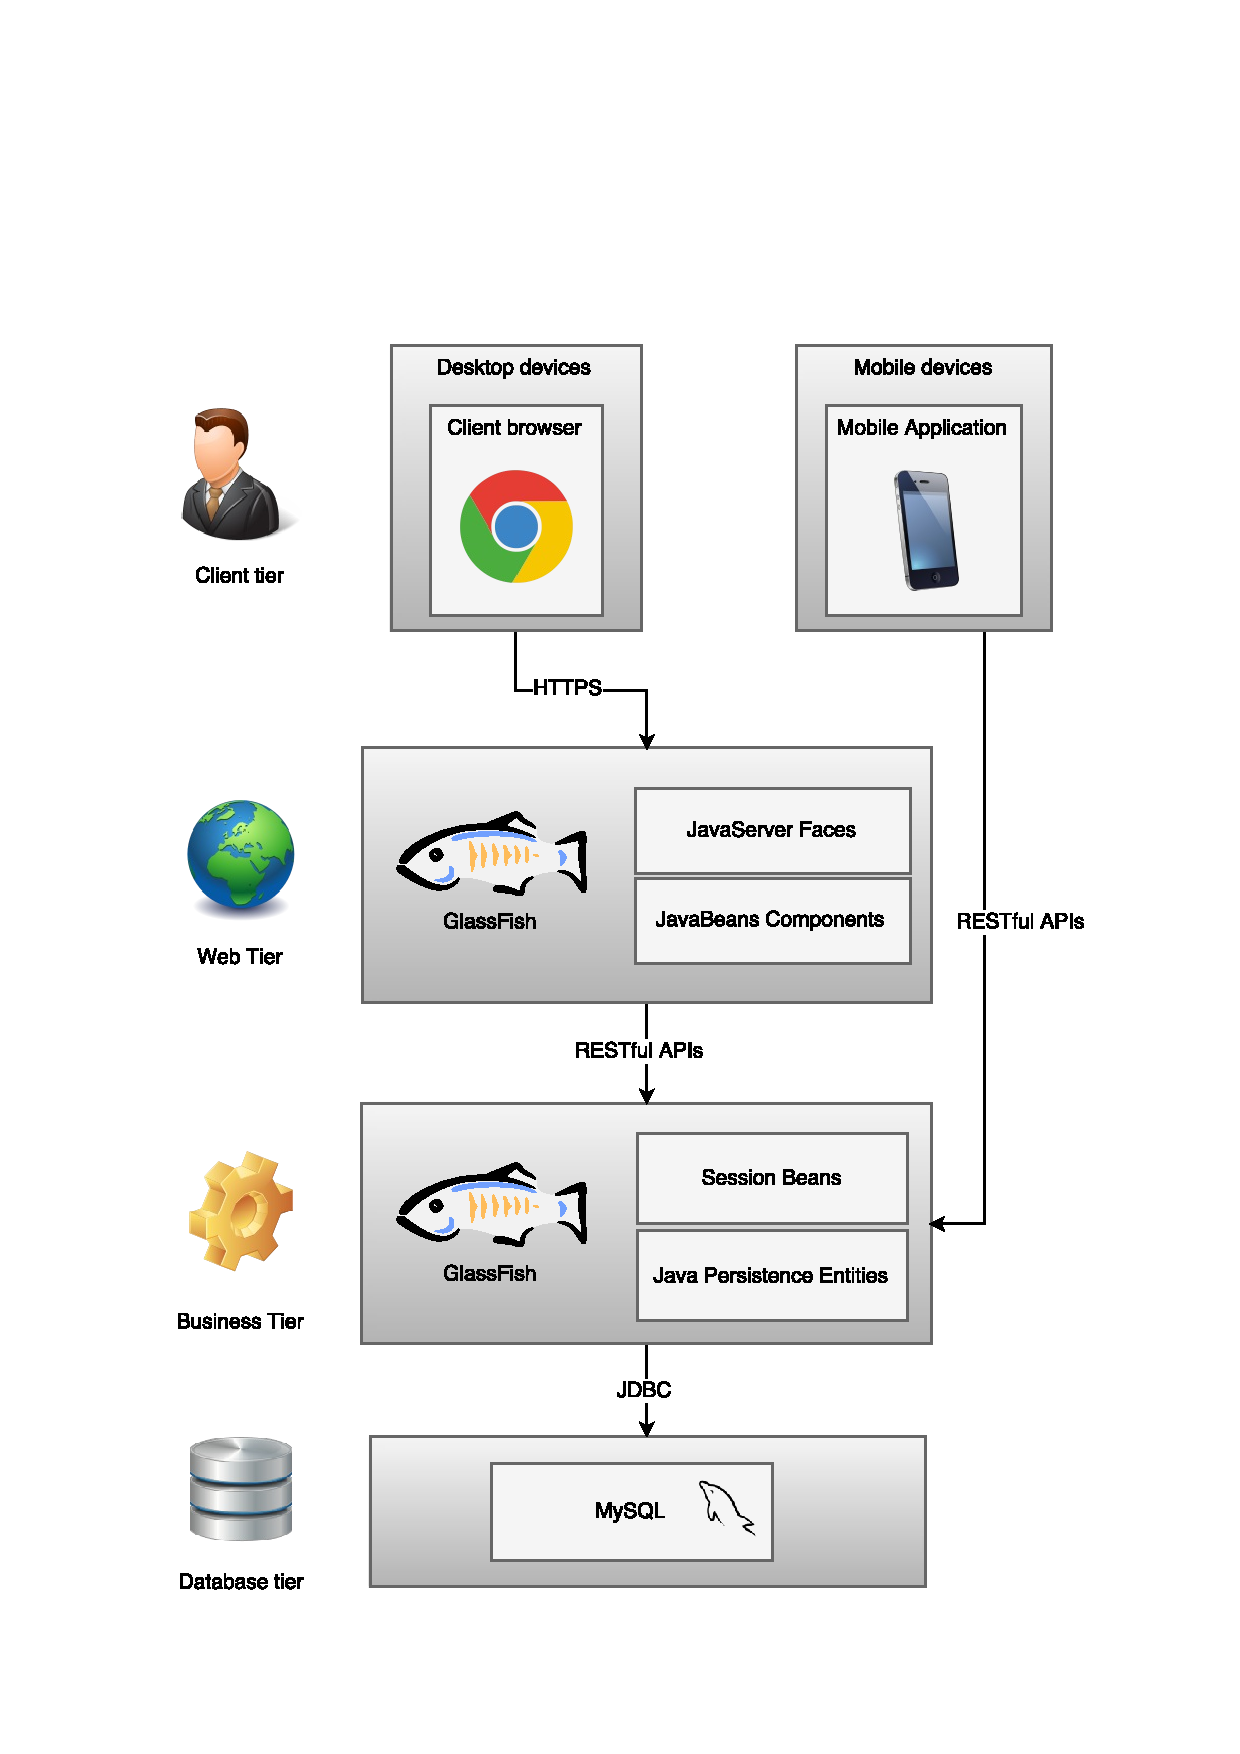
\includegraphics[width=\textwidth]{diagrams/JEE_Tiers}
\caption{The detailed description of tiers, detailed with JEE components.}
\label{fig:tiers-jee}
\end{figure}

\subsection{Database}
The database tier runs MySQL Community Edition and uses InnoDB as the database engine: the DBMS has to support transactions and ensure ACID properties.
The DBMS does not require specific design because it's an external component used as a ``black box'': the database only needs to be configured and tuned in the implementation phase.

The database can communicate only with the business logic tier using the standard network interface, described in \autoref{sec:component-interfaces}.
Security restrictions will be implemented to protect the data from unauthorized access: the database must be physically protected and the communication has to be encrypted. Access to the data must be granted only to authorized users possessing the right credentials. Every software piece that needs to access the DBMS must do so with the minimum level of privilege needed to perform the operations.

All the application data which needs to be persistent is stored in the database. The structure of the tables is illustrated by the E-R diagram in~\autoref{fig:er-diagram}.

\begin{figure}
    \centering
    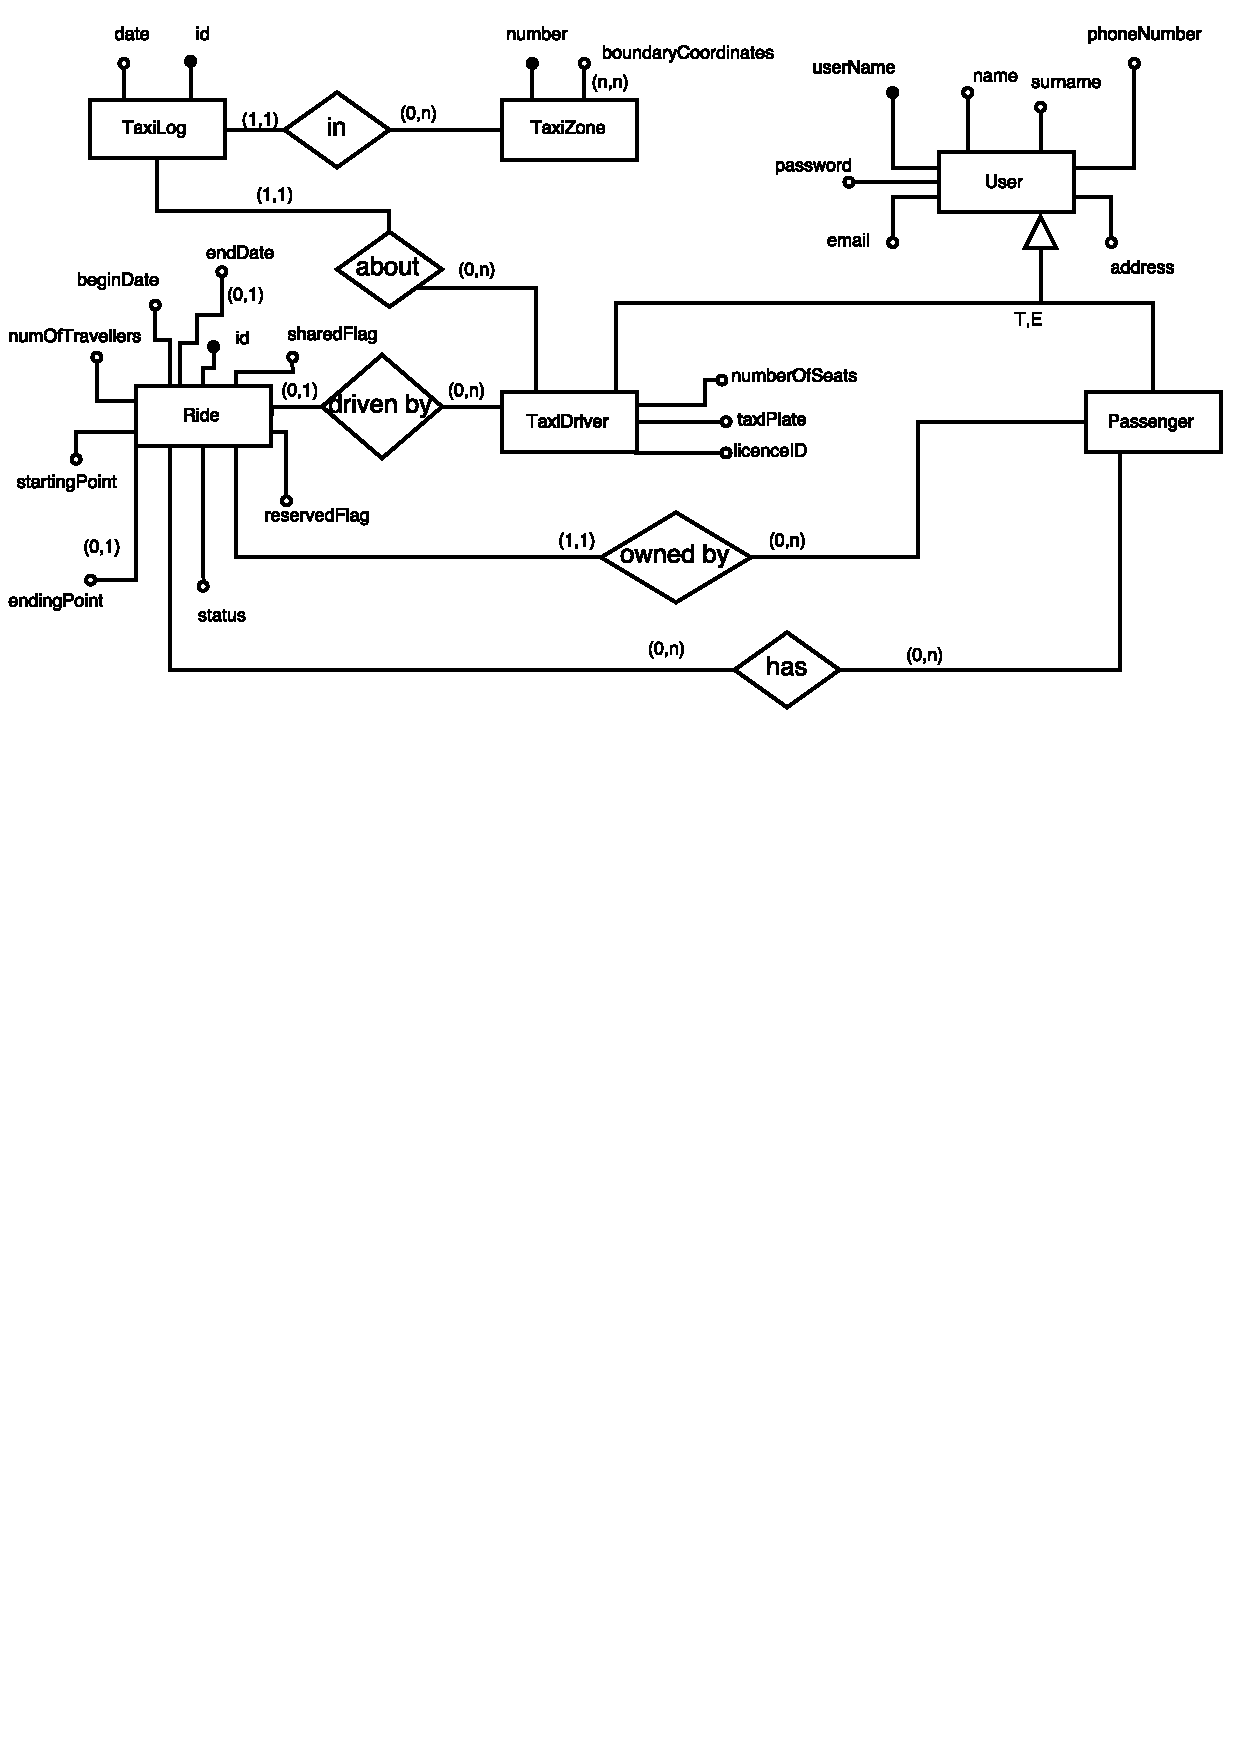
\includegraphics[width=\textwidth]{diagrams/er_diagram}
    \caption{The Entity-Relationship diagram of the database schema.}
    \label{fig:er-diagram}
\end{figure}

Foreign key constraints are used to guarantee some level of data integrity among the tables.
Triggers are not used: the dynamic behaviour of the data is handled entirely by the Java Persistence API in the Business Application tier.

\subsection{Application server}
The application server is implemented in the business logic tier, entirely written in Java EE and run by GlassFish Server.

Access to the database tier is not implemented with direct SQL queries: instead, it's completely wrapped by the \textbf{Java Persistence API (JPA)}. The object-relation mapping is done by entity beans.

The Entity Beans representing the database entities are strictly related to the entities of the ER diagram (\autoref{fig:er-diagram}). They are shown in~\autoref{fig:entity-diagram}.

\begin{figure}
    \centering
    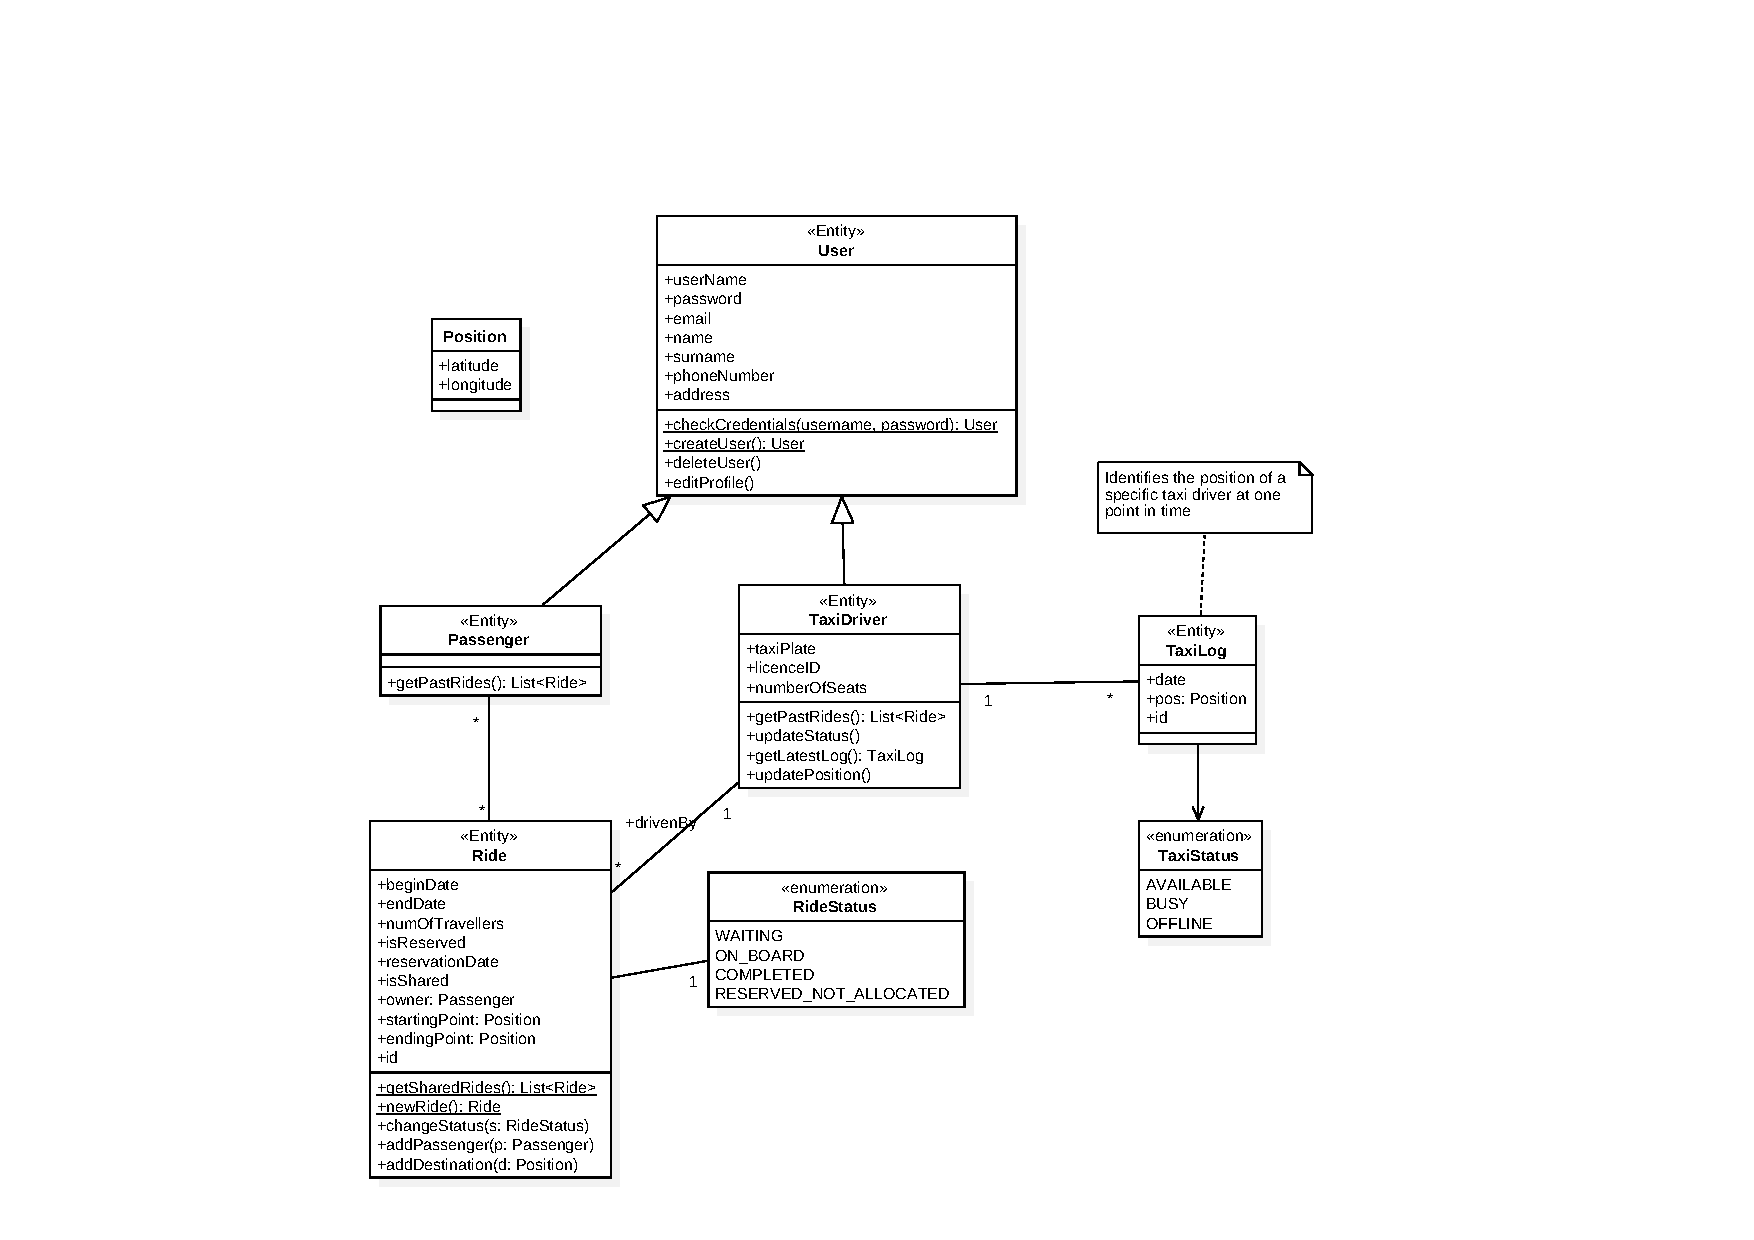
\includegraphics[width=\textwidth]{diagrams/entity_diagram}
    \caption{Java Entity Beans used to represent the entities in the database.}
    \label{fig:entity-diagram}
\end{figure}

The business logic is handled by \textbf{stateless Enterprise JavaBeans (EJB)}.
Our application indeed is rather simple and message-driven: the state of the users is stored in the DB, so we do not generally need stateful EJB which can be more expensive.
Concurrency management and performance is a great deal for this application, so the reusal of EJBs for many request is a desirable behaviour.

The application server implements a RESTful API using JAX-RS to allow the clients (web tier and mobile client) to use the services offered by the EJBs.

Session Beans used for the application server are shown in~\autoref{fig:session-beans}.

\subsubsection{UserManager}
This bean manages all the features related with user login, registration and profiles.
It implements user login, user registration, user deletion and user profile editing.
It also provides a function to confirm the email address provided by the user with the token sent by email.

\subsubsection{RideManager}
This bean creates new rides, assigns passengers and taxi driver to an existing ride and fetches information about rides.
It also allows taxi driver to update the status of a ride, signaling when the passengers are on board and when the ride is finished.

\subsubsection{TaxiManager}
This bean handles the taxi zones, their queues and the availability status and the position of taxi drivers.
Taxi drivers can mark themselves as available or unavailable, and they can change their position as well.

This component also has a method to find the first taxi in the queue for a specific taxi zone.

\subsubsection{HistoryManager}
This bean allows users (passengers and taxi drivers) to fetch the history of their rides.
It's able to store and retrieve the ended rides.

\subsubsection{EmailSender}
This bean is in charge of sending emails to users when needed. For now its only functionality is to send the e-mail confirmation token to the user e-mail address after the registration, but it could be extended to implement e-mail notifications.

\subsubsection{SharedRidePlugin}
This plugin implements all the functions related to the taxi sharing feature.
It allows the passengers to look for feasible shared rides and join them.

\subsubsection{ReservedRidePlugin}
This plugin implements all the functions related to the ride reservation feature.
Its function is to allow passenger to reserve a taxi for a future time.

\subsubsection{ConfiguratorBean}
This bean is a singleton and its only duty is to read the server configuration file and provide the value of configuration options. Other beans can ask for configuration options using the same keys used to define the settings in the configuration file.

\begin{figure}
    \centering
    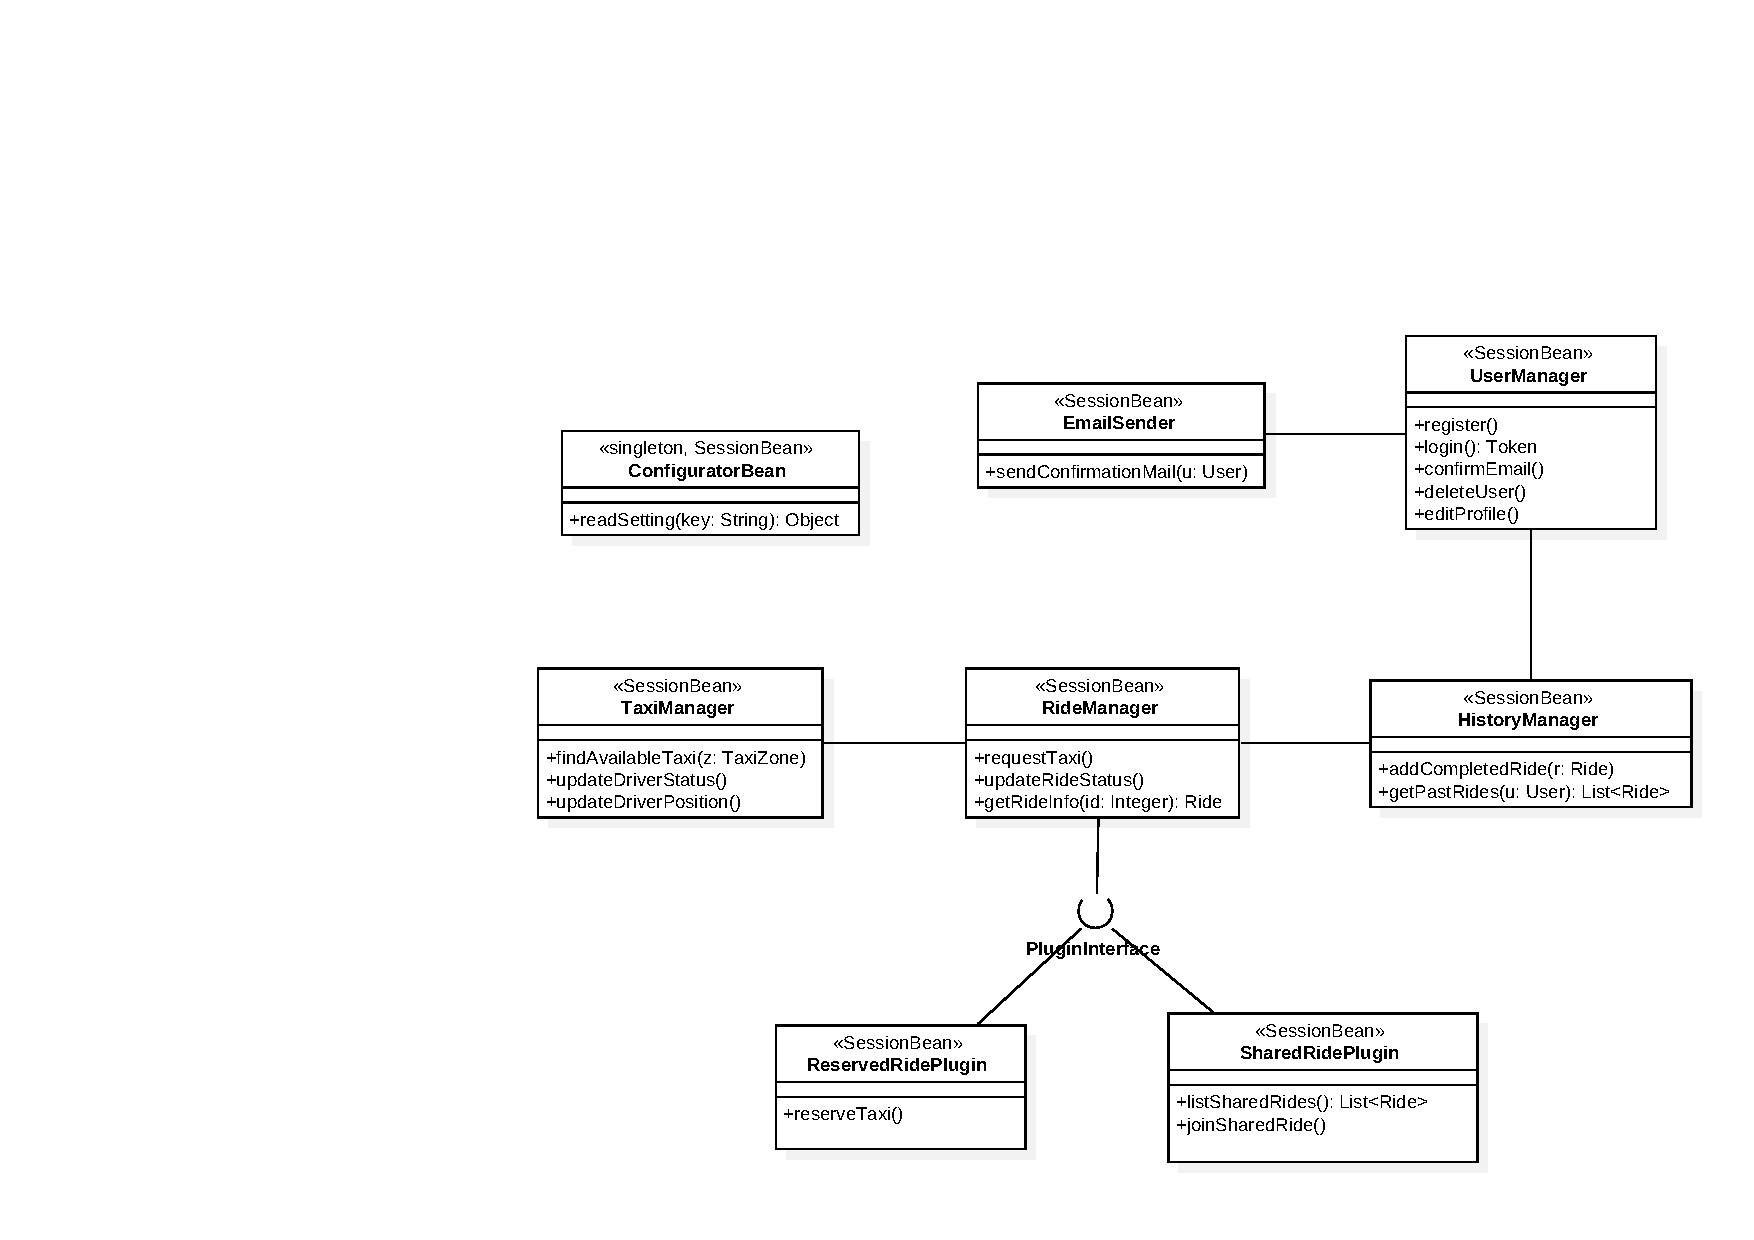
\includegraphics[width=\textwidth]{diagrams/class_sessionbeans}
    \caption{The session beans used in the implementation of the business logic. The parameters of the methods aren't written here: the detailed interface of each bean is described in detail in~\autoref{sec:rest-api}}.
    \label{fig:session-beans}
\end{figure}

\subsection{Web server}
The web server is implemented using Java EE web components to handle the presentation layer, namely JavaServer Faces (JSF), which is a server-side framework based on MVC.
The web server is run by GlassFish Server.

The web tier only handles the presentation layer: all the business logic is handled by the application server tier. The web tier uses the RESTful interface of the application tier.

Thanks to JSF, the view is written as XML files and is completely separated from the ``application logic'' of the web server. This enables us to write a modular web service.

\subsection{Mobile client}
% TODO mobile client design (Alex)
